\documentclass[uplatex,12pt]{jsarticle}
\usepackage[dvipdfmx]{graphicx}
\usepackage{url}
\usepackage{listings,jlisting}
\usepackage{ascmac}
\usepackage{amsmath,amssymb}

%ここからソースコードの表示に関する設定
\lstset{
  basicstyle={\ttfamily},
  identifierstyle={\small},
  commentstyle={\smallitshape},
  keywordstyle={\small\bfseries},
  ndkeywordstyle={\small},
  stringstyle={\small\ttfamily},
  frame={tb},
  breaklines=true,
  columns=[l]{fullflexible},
  numbers=left,
  xrightmargin=0zw,
  xleftmargin=3zw,
  numberstyle={\scriptsize},
  stepnumber=1,
  numbersep=1zw,
  lineskip=-0.5ex
}
%ここまでソースコードの表示に関する設定

\title{知能プログラミング演習II 課題2}
\author{グループ8\\
  29114116 増田大輝\\
}
\date{2019年10月7日}

\begin{document}
\maketitle

\paragraph{提出物} rep2
\paragraph{グループ} グループ8

\paragraph{メンバー}
\begin{tabular}{|c|c|c|}
  \hline
  学生番号&氏名&貢献度比率\\
  \hline\hline
  29114003&青山周平&NoData\\
  \hline
  29114060&後藤拓也&NoData\\
  \hline
  29114116&増田大輝&NoData\\
  \hline
  29114142&湯浅範子&NoData\\
  \hline
  29119016&小中祐希&NoData\\
  \hline
\end{tabular}



\section{課題の説明}
\begin{description}
\item[課題2-1] MatchingクラスまたはUnifyクラスを用い,パターンで検索可能な簡単なデータベースを作成せよ.
\item[課題2-2] 自分たちの興味ある分野の知識についてデータセットを作り,上記2-1で実装したデータベースに登録せよ.また,検索実行例を示せ.どのような方法でデータセットを登録しても構わない.
\item[課題2-3] 上記システムのGUIを作成せよ. \\
・データの追加,検索,削除をGUIで操作できるようにすること. \\
・登録されたデータが次回起動時に消えないよう,登録されたデータをファイルへ書き込んだり読み込んだりできるようにすること.
\end{description}

\section{課題2-3}
\begin{screen}
    上記システムのGUIを作成せよ.\\
    ・データの追加,検索,削除をGUIで操作できるようにすること. \\
    ・登録されたデータが次回起動時に消えないよう,登録されたデータをファイルへ書き込んだり読み込んだりできるようにすること.
\end{screen}
\noindent
私の担当は全体のシステム設計とPresenterの構築に留まるため,実行例は無い. \\
実装と考察に関しては適宜,各種手法の詳細説明において言及する. \\
また,必要に応じてソースコードを明示する場合もある. \\

\subsection{手法}
今回の課題では,データベースの利用やGUIの設計などシステムを構成する要素が前回課題よりも多いと考えられる.
したがって,機能区分を明確に行うことによって,システムとしての保守性やソースコードの可読性,依存関係の明確化を狙うことが重要であると考えた.
これらの目的を達成するために,以下のような一般的にシステム・アプリケーション開発で取り入れられている設計概念を採用することとした.
\begin{description}
    \item[MVPアーキテクチャ]
    \item[DAOパターン]
    \item[抽象化による疎結合な関係性の構築]
\end{description}

\subsection{MVPアーキテクチャの導入}
課題2-3では,GUIの使用やデータベースの応用が必要となるため,明確な機能区分を与えることで全体の設計指針が立つと考えられる.
そこで,今回はアプリケーションアーキテクチャとして代表的なMVPアーキテクチャを採用することによって,機能の切り分けを行った.
以下にMVPアーキテクチャの各構成要素について述べる.
\begin{description}
\item[Model] データ処理機構を担っている.今回はデータを格納するデータベースやデータベースへのアクセスを担うDAOが該当する.ViewやPresenterに依存しない.
\item[Presenter] Viewから受けた処理に基づいてModelからデータを取得し,画面反映を行うためのViewメソッドを呼び出す.これにより,ViewとModel間の円滑なデータフローと画面制御を行う.
\item[View] ユーザーインターフェースを担う.ユーザー入力を受け取り,Presenterに通知し,処理結果を出力として画面に表示する.今回は,入出力に対応するロジックで構成されるGUIが該当する.
\end{description}
以下にMVPアーキテクチャの概念図を示す.
\begin{figure}[!hbt]
    \centering
    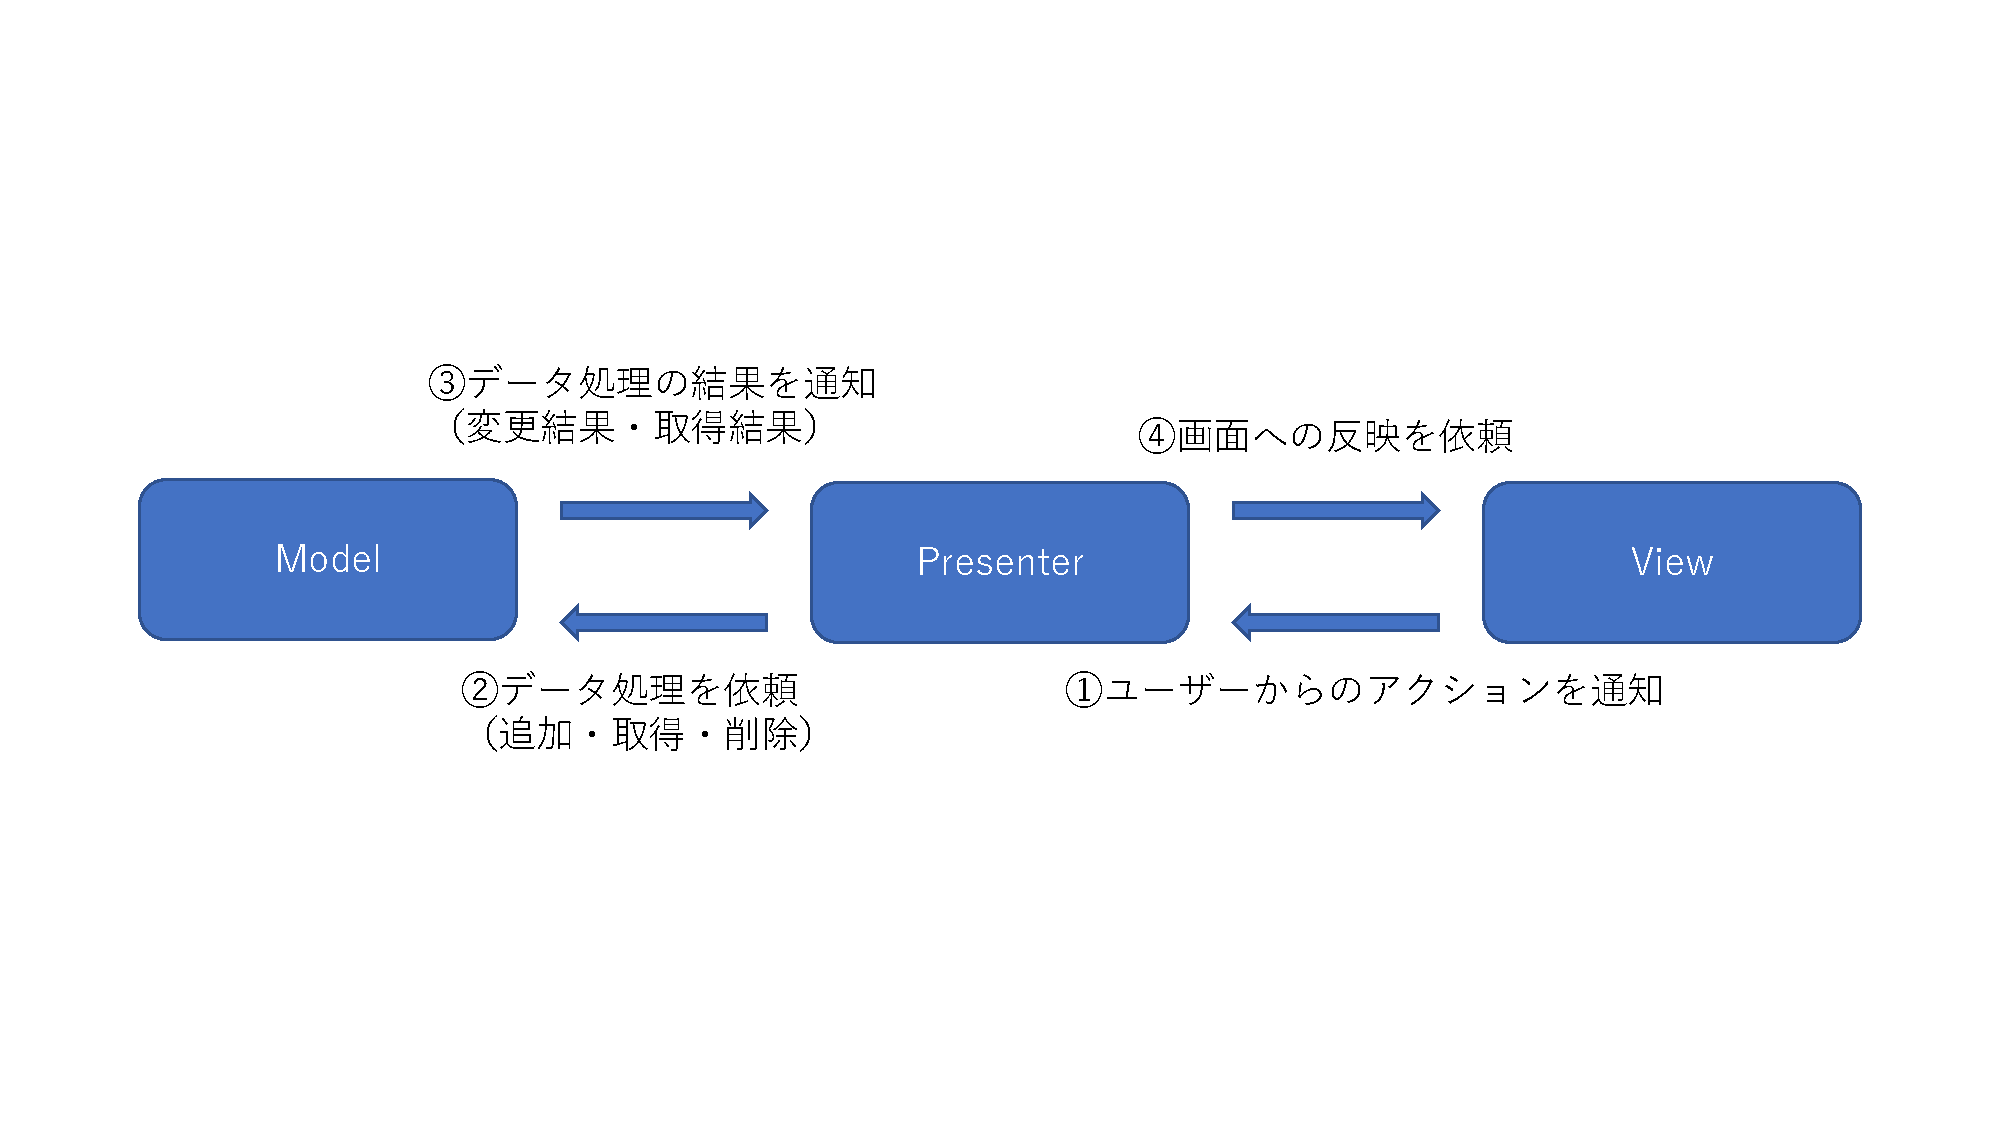
\includegraphics[scale=0.35]{images/mvp_architecture.pdf}
    \caption{MVPアーキテクチャの概念図}
\end{figure}


\subsection{DAOパターンの導入}
今回は,データベースへのアクセスを一括して担うデザインパターンであるDAOを導入した.
全てのデータ処理において,必ずDAOを通すことによって,他のクラスにデータベースアクセスメソッドが分散することを防ぐことができる.
さらに,Modelとしての機能を担っていると考えられるため,PresenterのみがDAOインスタンスを握るように設計した.
ただし,テキストファイルの使用が課題の条件として提示されていたため,通常アプリケーション開発では行われないテキストファイル-データベース間の処理機構も必要となった.
これに対処するために,今回は通常のDAOに加え,テキストファイル-データベース間の処理を担当するTextDAOを設計した.
これら二種類のDAOの分類は,以下の考えに基づいて明確に規定される.
\begin{description}
\item[DAO] 通常のデータベースアクセス処理を担い,今回はデータの追加・取得・削除を行うメソッドを取りまとめている.
\item[TextDAO] データベースをテキストファイルの一次キャッシュとみなし,テキストファイル-データベース間の読み書きを担当する.具体的には,GUI起動時にテキストファイルからデータベースへのデータを読み込み,GUI終了時にデータベースからテキストファイルへのデータ書き込みを行う.結果として,テキストファイルとデータベースの一貫性を保つこととなる.
\end{description}
以下にDAOパターンの概念図を示す. \\
\begin{figure}[!hbt]
    \centering
    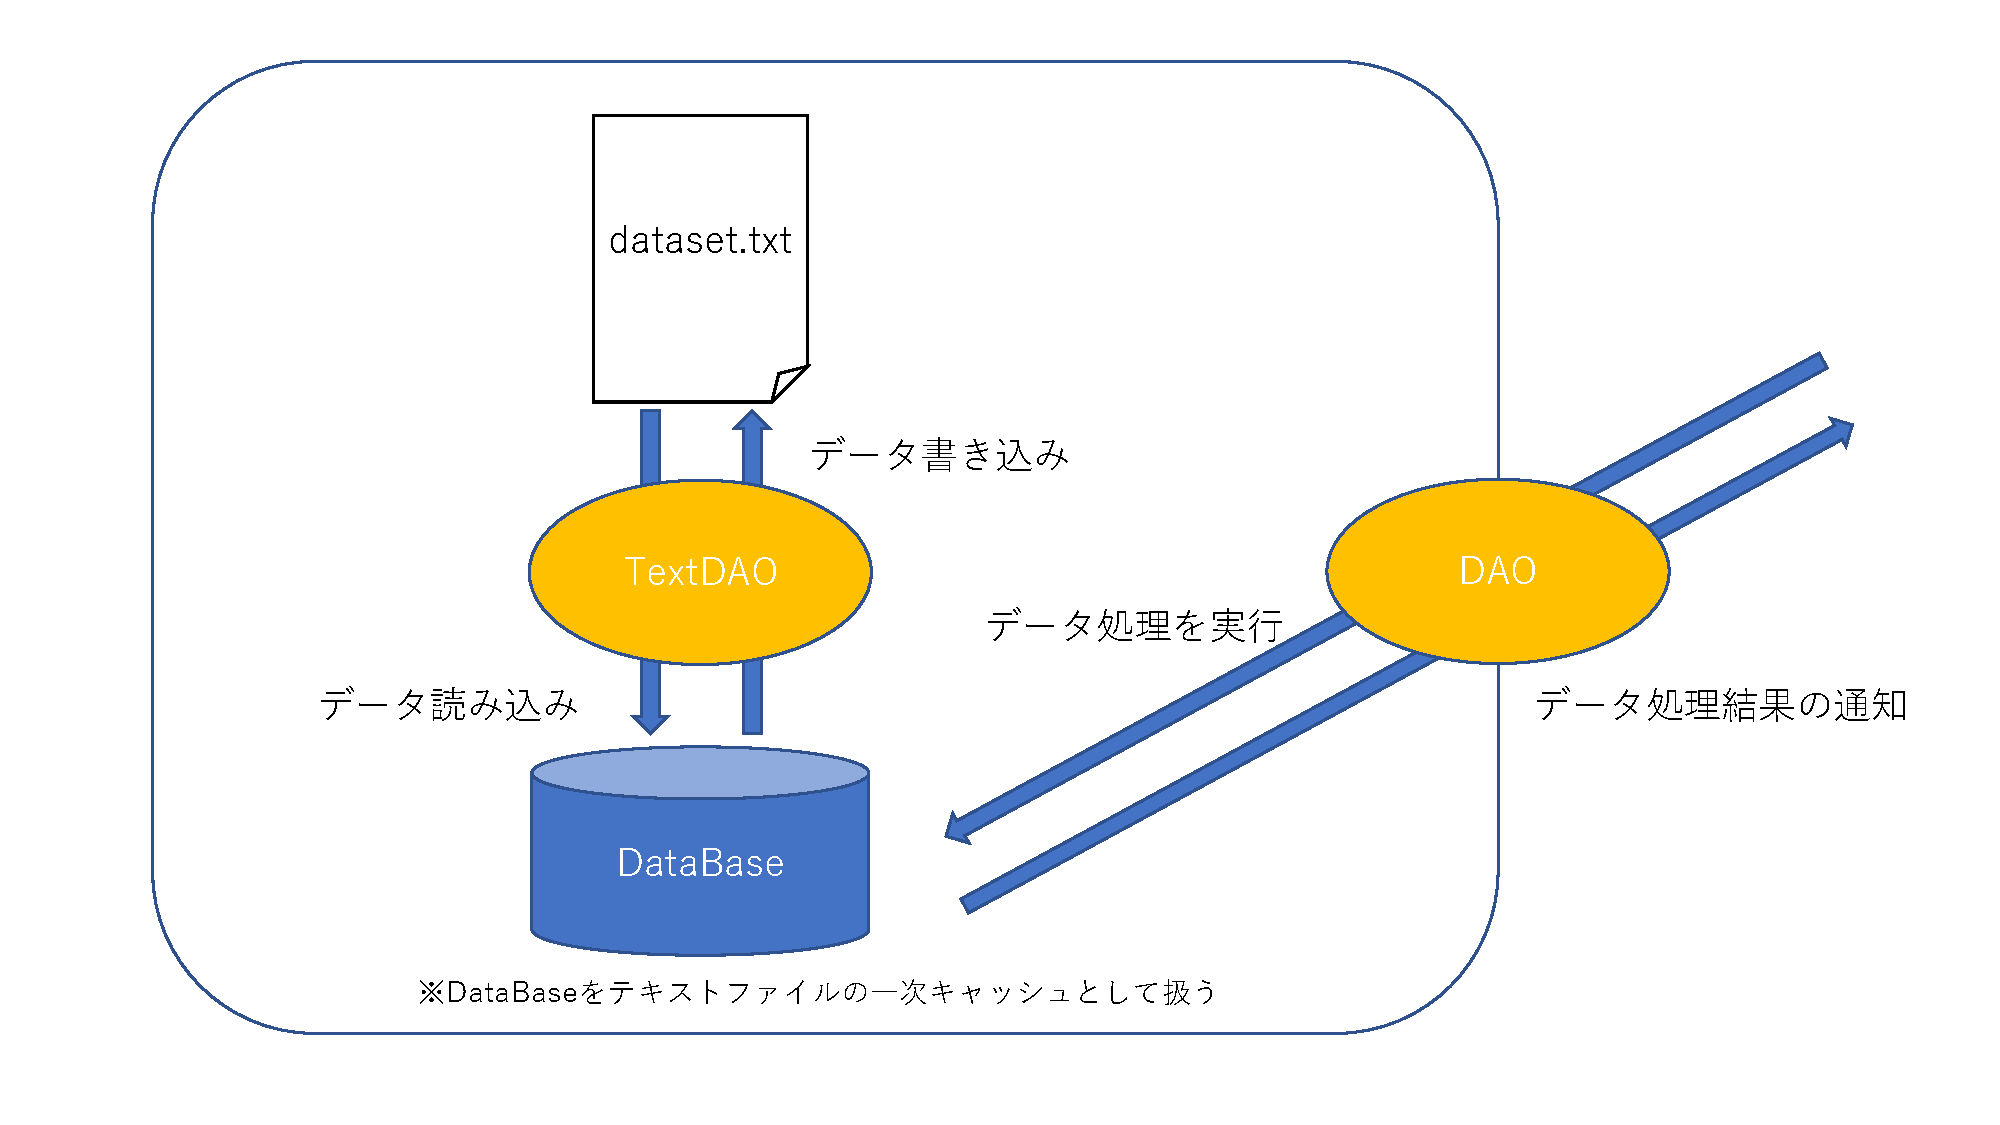
\includegraphics[scale=0.35]{images/dao_pattern.pdf}
    \caption{DAOパターンの概念図}
\end{figure}

\noindent
今回,PresenterはTextDAOに対して以下のメソッドを要求する.
\begin{description}
    \item[readTextFileメソッド] テキストファイルからデータベースへのデータ読み込み
    \item[writeTextFileメソッド] データベースからテキストファイルへのデータ書き込み
\end{description}
PresenterはDAOに対して以下のメソッドを要求する.
\begin{description}
    \item[addDataメソッド] データベースにデータを追加する
    \item[fetchDataListメソッド] データベースからデータを取得する
    \item[deleteDataメソッド] データベースからデータを削除する
\end{description}

\subsection{抽象化による疎結合な関係の構築}
まず,MVPアーキテクチャにおける各要素の間の依存関係について述べる.
上述した通り,ModelクラスはPresenterやViewに全く依存していない.
一方で,PresenterがModelインスタンスを握っていることから,PresenterはModelに依存する関係にある.
加えて,MVPアーキテクチャ含め,一般的なMVC系統のアーキテクチャにおいては,ViewがController部のインスタンスを握ることから,今回はViewがPresenterインスタンスを握ることとなる. \\
ここで,MVPアーキテクチャの特徴として,Presenterはユーザー入力をModelに通知するだけで無く, 直接Viewへの反映命令を行う点があげられることに注目する.
後者の機能の実現には,何らかの形でPsesenterからViewメソッドを呼び出す必要性が生じる.
したがって,Presenter内において,Viewメソッドを持ちうるインスタンスの生成が不可避的となる. \\
しかし,ViewとPresenterが直接互いのインスタンスを握り合うことは望ましく無い.
何故ならば,これらの要素が互いのインスタンスをにぎり合うことにより,強結合と呼ばれる相互的な依存関係が生まれ,アーキテクチャを採用することによる機能分割の意味が薄れるためである.
実際,互いに直接インスタンスを握り合うのであれば,アーキテクチャという観点からはクラスを統一した場合と意義的にはほぼ等しい. \\
この問題を解決するための手法が,インターフェースを利用した抽象化による疎結合な関係の構築である.
実装としては,PresenterからViewを管理するメソッドを集めたViewInterfaceを定義し,Presenter側ではViewInterface型インスタンスを持つようにする.
\begin{lstlisting}[caption=ViewInterfaceの定義, label=mid]
    interface ViewInterface {
        \\データベース初期化完了メソッド
        void successStart();
        \\テキストファイル記録完了メソッド
        void successFinish();
        \\データ追加完了メソッド
        void successAddData();
        \\検索結果反映メソッド
        void showSearchResult(List<TextModel> resultList);
        \\データ削除メソッド
        void successDeleteData();
        \\一覧表示メソッド
        void showResultList(List<TextModel> resultList);
        \\例外処理表示メソッド
        void showError(String errorText);
        \\データ無し表示メソッド
        void showNoData();
    }
\end{lstlisting}
\begin{lstlisting}[caption=PresenterにおけるViewInterface型インスタンスの生成, label=mid]
    class Presenter {
        ...
        private ViewInterface view;

        public Presenter(ViewInterface view) {
            this.view = view;
        }
        ...
    }
\end{lstlisting}
View側の実装クラスでは,インターフェースを実装し,オーバーライドされたメソッドの具体的な処理を記述する.
\begin{lstlisting}[caption=GUIにおけるPresenterインスタンス生成, label=mid]
    class GUI implement ViewInterface {
    ...
    Presenter presenter;
    init() {
        presenter = new Presenter(this);
    }
    ...
}
\end{lstlisting}
また,Viewは生成後にPresenterコンストラクタに自身を渡すことで,Presenterインスタンスを生成する.
反対にViewの終了時には,Presenterインスタンスを離すように設計する. \\

以上により,ViewがPresenterインスタンスを握ることで依存しながらも,Presenter側は直接明示的にViewインスタンスを握らずともViewメソッドを呼び出せる状態が完成する.
すなわち,ViewがPresenterを持つという一方的な依存関係としての疎結合な関係の構築が達成される. \\
結果的に,一般的にアーキテクチャを採用する際に好ましいとされる緩やかな関係性を持たせることができるのである. \\
以下に,View-Presenter間における疎結合な関係を示す.
\begin{figure}[!hbt]
    \centering
    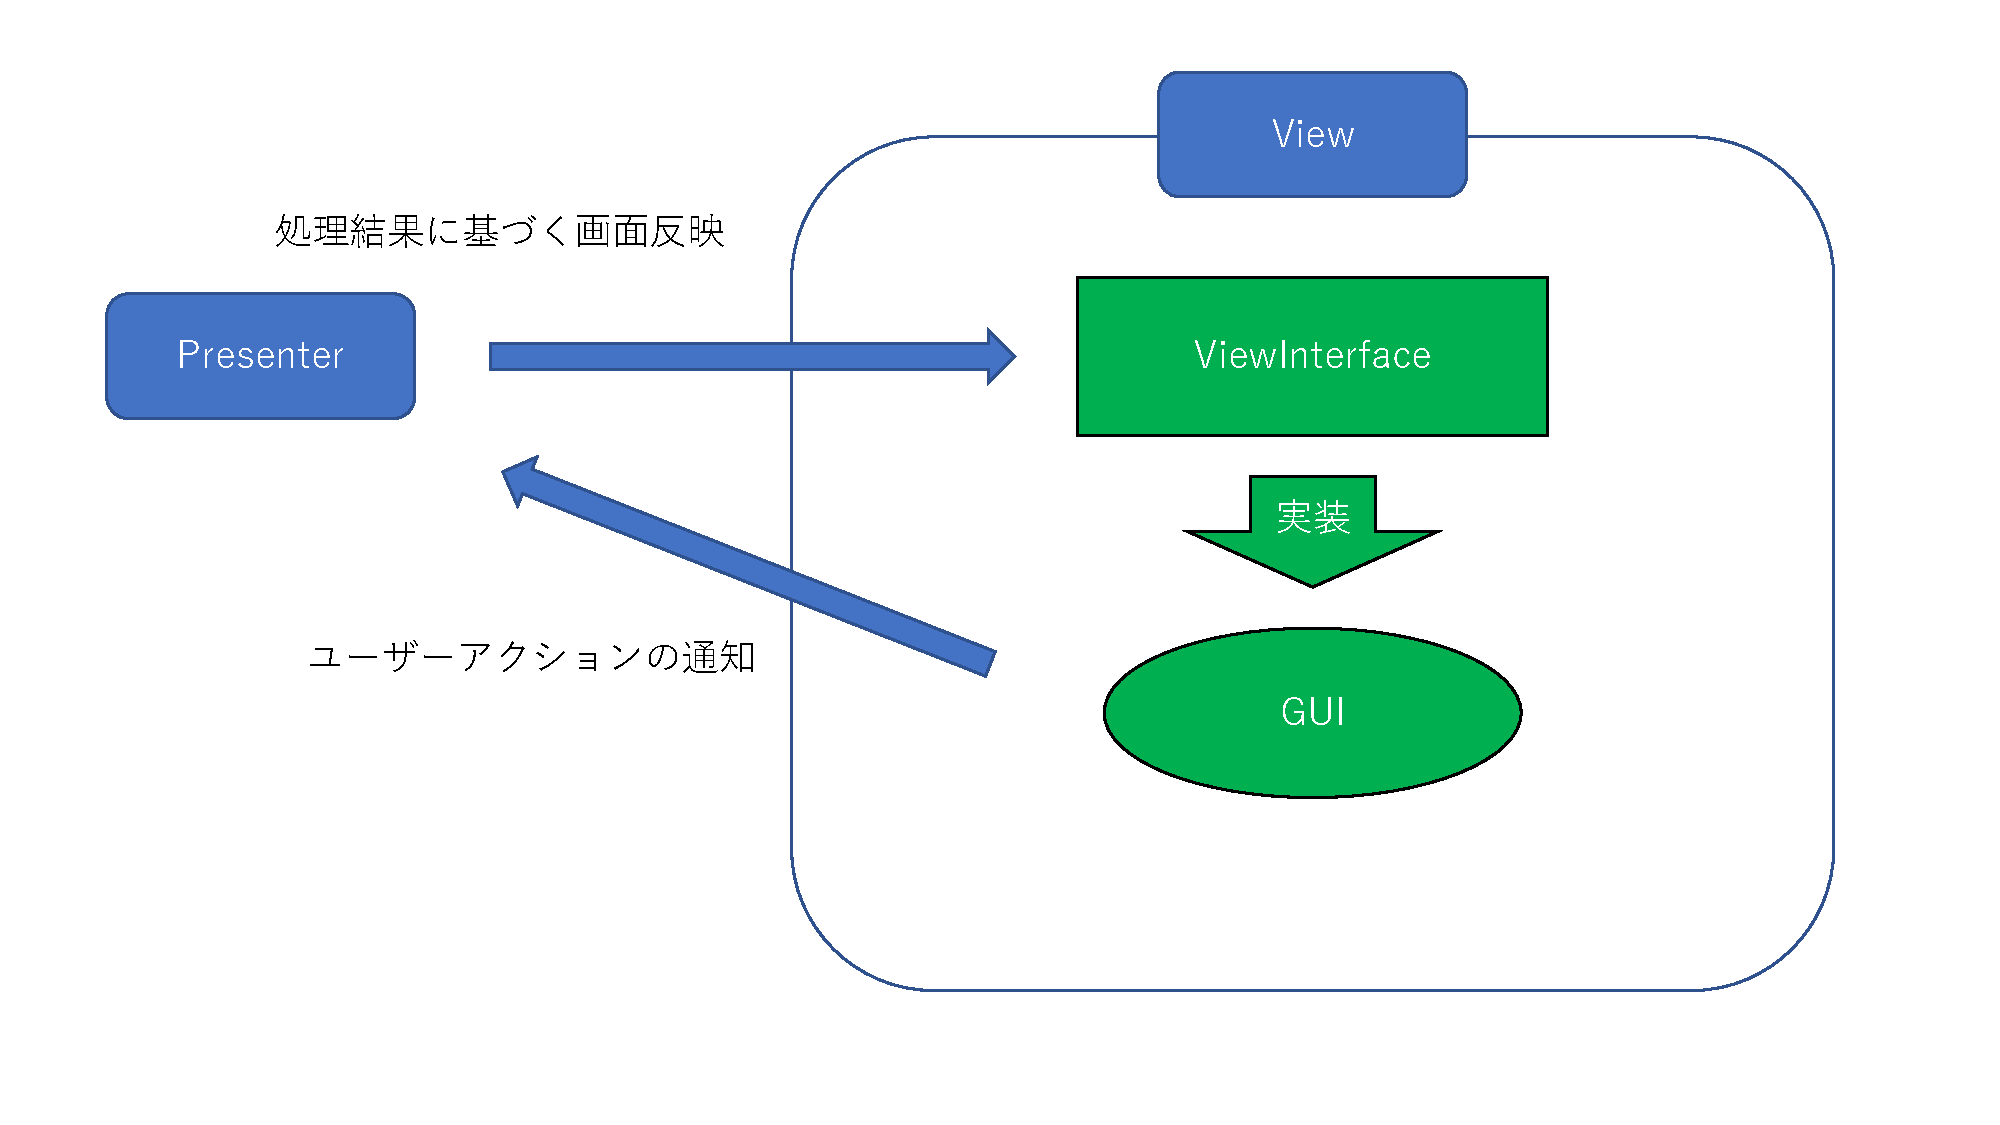
\includegraphics[scale=0.35]{images/view.pdf}
    \caption{View内部とPresenterの依存関係の概念図}
\end{figure}

\newpage

\subsection{システムの全体像}
上述した3種類の技術を用いて,今回の課題のシステムを実現した.
その全体像を以下に示す.
\begin{figure}[!hbt]
    \centering
    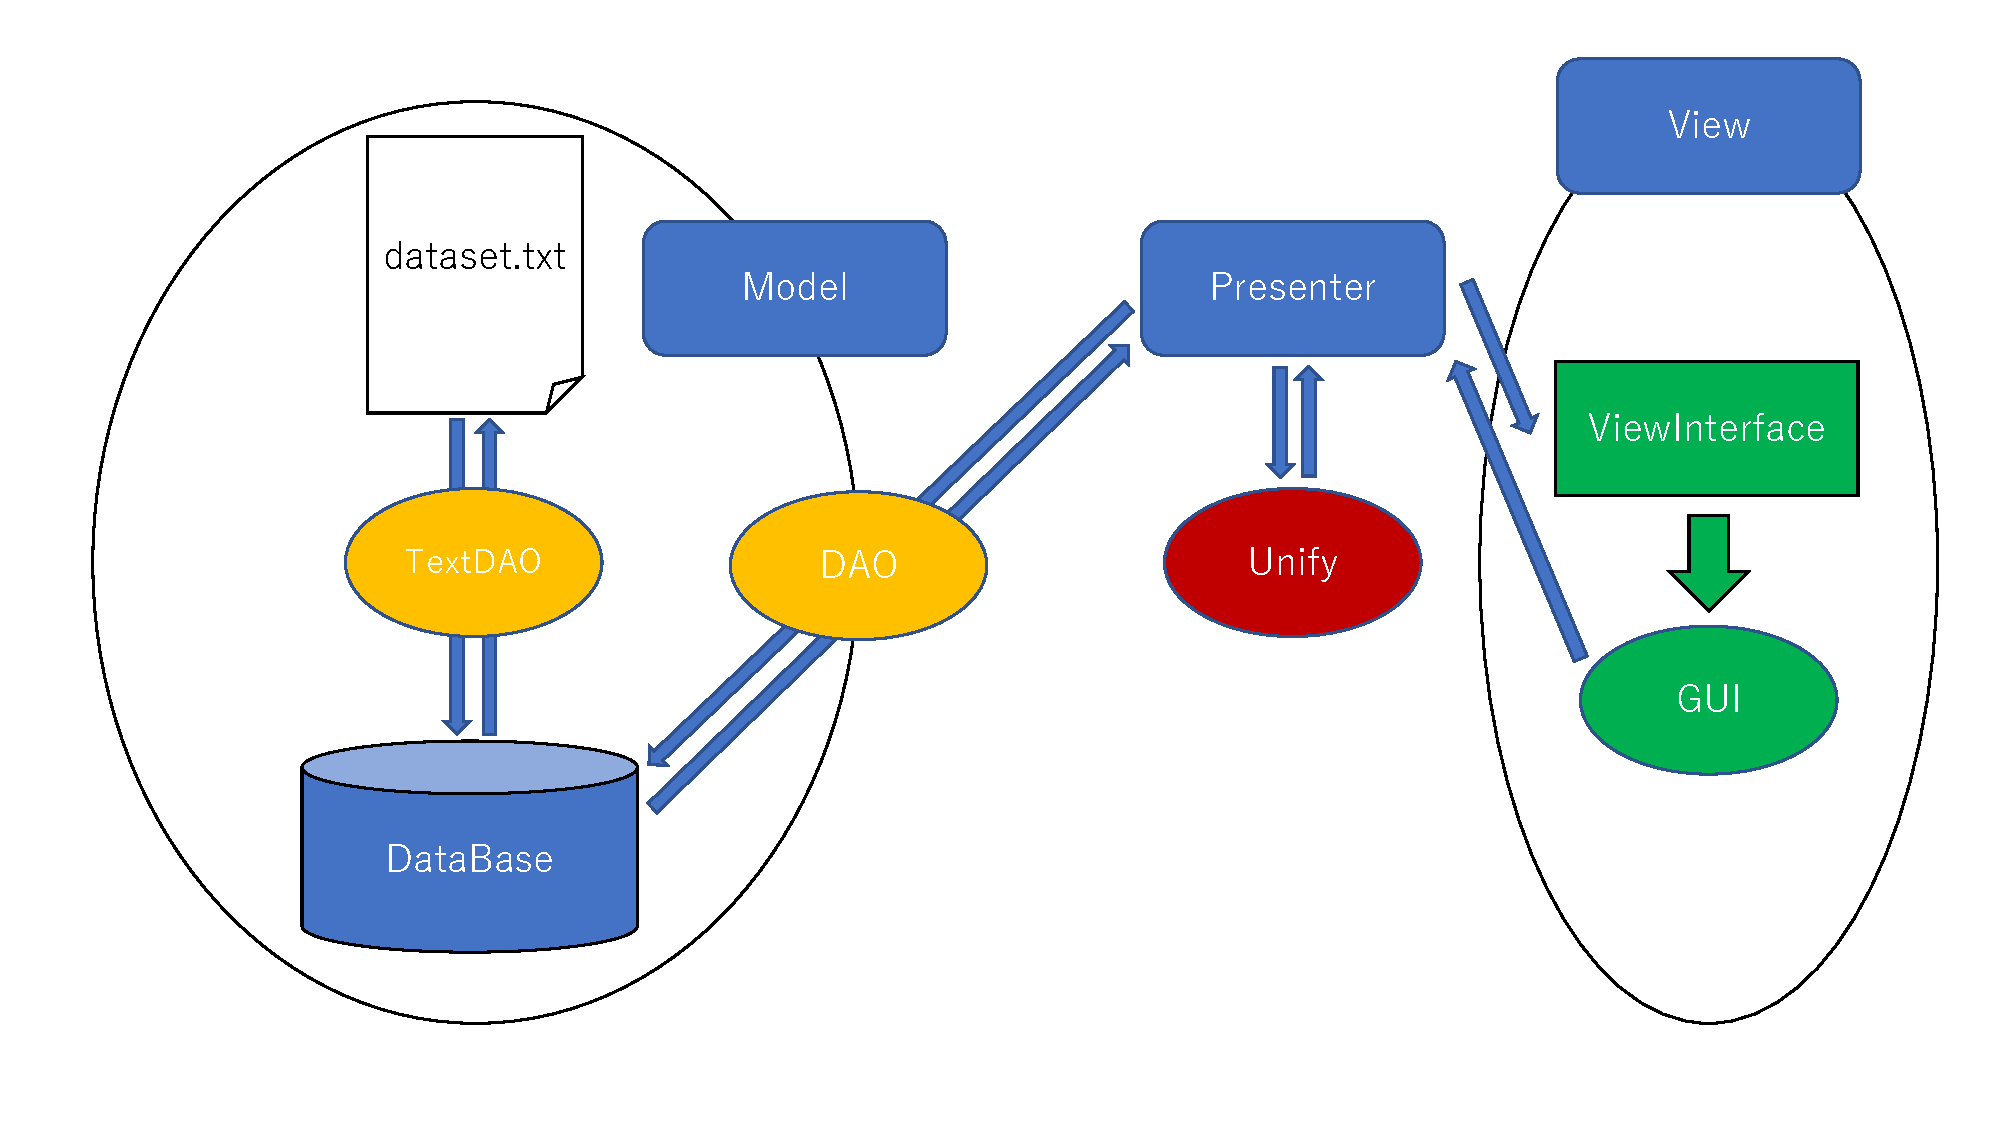
\includegraphics[scale=0.35]{images/architecture_all.pdf}
    \caption{システム全体の概念図}
\end{figure}

\subsection{データ追加・削除機能の実装}
Viewがユーザー入力を受け取り,Presenterに通知する.
PresenterはDAOに問い合わせ,結果により呼び出すViewメソッドを切り替えてViewに反映指示を出す.

\subsection{データ検索・一覧表示機能の実装}
Viewがユーザー入力を受け取り,Presenterに通知する.
PresenterはDAOに問い合わせ,結果として受け取ったデータリストとユーザー入力から得られた文字列をUnify内部のメソッドに渡すことで検索を行う.
Unifyによる検索結果から,呼び出すViewメソッドを切り替えてViewに反映指示を出す.

\subsection{テキストファイル-データベース間の読み込み/書き込み機能の実装}
Viewがユーザー入力を受け取り,Presenterに通知する.
PresenterはTextDAOに問い合わせ,実行結果により呼び出すViewメソッドを切り替えてViewに反映指示を出す.


\subsection{考察}
ここでは,全体的な考察について述べることとする. \\
まず,アプリケーション/システムとして重要なのは機能を明確に区分することであると考えた.
次に,チーム開発を行うに当たって,保守性や可読性を高めることに重点を置くべきだと考えた.
これら二つの考えを基として,MVPアーキテクチャやDAOパターンの導入が適切であると判断した.
その反面,概念的な要素が多く,チームメンバーに対しての説明を要した.
しかし,GitHub上でソースコード管理を行っているので,コンフリクションを防止するためにもアーキテクチャやデザインパターンにより役割分担を行うことは非常に有効な手段であると考えられる. \\

さて,機能の切り分けと分担を考える上では非常に良い課題であると感じた反面,今回の課題について,非常に違和感を感じた点がある.
それは,課題2-3において,テキストファイルへのデータ読み込みと書き出しによりデータの保管を行う指示があることだ.
私は,今までAndroidアプリケーションの開発に携わってきたが,まずデータ保管のためにテキストファイルを用いるのは一般的では無いとの認識を持っている.
通常,サーバーに管理を任せるか,OS標準搭載のデータベースを用いる.
今回であれば,課題2-1でデータベースの作成を要求されているので,データベースを利用するのみで十分であると考えられる.
また,データベースの永続性の観点から,わざわざテキストファイルへの保存を行うのは冗長であると感じられる.
課題の指示内容の解釈に苦しんだので,グループメンバーがTAに質問して提案された内容を重んじ,データベースをテキストファイルの一次キャッシュのような形にすることを決定した.
上述した通り,データベースの利用法としては非常にナンセンスだと感じられる. \\
次に,Unifyとデータベースの検索機能が競合する点である.
Unifyは読み込んだデータを元に指定された文字列とのマッチングを行うことで検索を行う.
一方で,データベースに動詞ごとのテーブルを作り,主格と目的格を属性として持たせ,SELECT文を実行することで同様の機能を実装できる.
すなわち,検索機能に関して二つの実装方式が可能であり,問題文からはUnifyを用いる実装,一般的にはデータベースを用いる実装があげられる.
前者を採用した場合は,データベースはただ一つのみのテーブルを持ち,そのまま文章を格納するだけの機能となり,十分にデータベースを活用できているとは言えない.
後者を採用した場合は,そもそもUnifyを利用する必要性が無くなり,課題の趣旨に反する可能性がある.
結果的に,今回の課題テーマにあるパターンマッチングを活かすために前者を採用したが,現実的な開発においては後者が最適であると個人的に強く感じる. \\
これらのような課題指示の曖昧性と現実的なシステムからの乖離は学生を非常に混乱させ,メンバー間の意思疎通をいたずらに困難とすると考えられる.
もちろん,実装課題であるので,受け手側の受け取り方による多少の揺らぎは許容されるべきであるが,学生の知識や経験にそぐわない実装を手段として選ばざるを得ないような表現にはいささか疑問が残る.
課題内容の吟味と説明の徹底を行うことを強く推奨すると共に,このように学生が解釈に手間取る可能性を十分に考慮して,課題内容を早期に公開すべきであると考える.


\subsection{感想}
以上のような疑問を抱えたまま,グループワークを行うと統制が取れなくなるだけでなく,システム設計者として大変苦労することが理解できた.
提出期限が約一週間という短期間であることを考慮すると、他メンバーの進捗等を考慮してなるべく早めに全体の方針を打ち出す必要があるので,急いで作業を行うようにしている.
結果的に,課題の曖昧性を吟味することやメンバーの理解状況の把握することに非常に骨が折れる.
さらに,今回の課題では,曖昧性の中でこのような実装を採用した根拠をメンバーに説明する義務が生じる.
そのために,徹夜を余儀なくされ,本来の予定をキャンセルするなど生活に実害が及んでいる.
もう一度強調したいが,極めて計画的に行動していてもこのような負担を強いられているのが現状である.
したがって,課題の出題方法・内容に対して非常に不満を感じた.



% 参考文献
\begin{thebibliography}{99}
\bibitem{notty} 新入社員におくるGitHubでのプロジェクト管理の初歩 --著:hayato ki \\
\url{https://qiita.com/gumimin/items/63dcb36d4730213bd63a} (2019年10月7日アクセス).

\end{thebibliography}

\end{document}